\documentclass[a4paper]{article}

\usepackage[utf8]{inputenc}
\usepackage[T1]{fontenc}
\usepackage{textcomp}
\usepackage{listings}
\usepackage{lmodern}
\usepackage{amsfonts}
\usepackage{titling}
\usepackage{lipsum}
\usepackage[left=1in, right=1in, bottom=1in, top=1in]{geometry}
\usepackage{amsthm}
\usepackage{tcolorbox}
\usepackage{hyperref}
\usepackage{xcolor}
\usepackage{graphicx}
\usepackage{makeidx}
\usepackage{tikz}
\usepackage{cases}
\usepackage{apacite}
\usepackage{tkz-berge}
\usepackage{url}
\usepackage{tgtermes}
\usepackage{sectsty}
\usepackage{subcaption}
\usepackage{setspace}
\usepackage{float}
\usepackage{amsmath, amssymb}


% figure support
\usepackage{import}
\usepackage{xifthen}
\pdfminorversion=7
\usepackage{pdfpages}
\usepackage{transparent}
\usepackage{color}
\newcommand{\incfig}[2][1]{%
    \def\svgwidth{#1\columnwidth}
    \import{./figures/}{#2.pdf_tex}
}

%mathstyling
\theoremstyle{plain}
\newtheorem{thm}{Theorem}[section]
\newtheorem{lem}[thm]{Lemma}
\newtheorem{prop}[thm]{Proposition}
\newtheorem*{cor}{Corollary}

\theoremstyle{definition}
\newtheorem{defn}{Definition}[section]
\newtheorem{conj}{Conjecture}[section]
\newtheorem{exmp}{Example}[section]
\newtheorem{axiom}{Axiom}
\theoremstyle{remark}
\newtheorem*{rem}{Remark}
\newtheorem*{note}{Note}

\definecolor{darkgreen}{rgb}{0.0, 0.5, 0.0}

\pdfsuppresswarningpagegroup=1
\lstset{
tabsize = 4, %% set tab space width
showstringspaces = false, %% prevent space marking in strings, string is defined as the text that is generally printed directly to the console
numbers = left, %% display line numbers on the left
commentstyle = \color{darkgreen}, %% set comment color
keywordstyle = \color{blue}, %% set keyword color
stringstyle = \color{red}, %% set string color
rulecolor = \color{black}, %% set frame color to avoid being affected by text color
basicstyle = \small \ttfamily , %% set listing font and size
breaklines = true, %% enable line breaking
numberstyle = \tiny,
  frame=none,
  xleftmargin=2pt,
  stepnumber=1,
  belowcaptionskip=\bigskipamount,
  captionpos=b,
  escapeinside={*'}{'*},
  language=haskell,
  tabsize=2,
  emphstyle={\bf},
  showspaces=false,
  columns=flexible,
  showstringspaces=false,
  morecomment=[l]\%,
}
\begin{document}
	\begin{titlepage}
	\begin{center}
	\large
	University of Warwick \\
	Department of Computer Science \\
	\huge
	\vspace{50mm}
	\rule{\linewidth}{0.5pt} \\
	CS126 \\
	\vspace{5mm}
	\Large
	Design of Information Structures
	\rule{\linewidth}{0.5pt}
	\vspace{5mm}
	\begin{figure}[H]
	\centering
	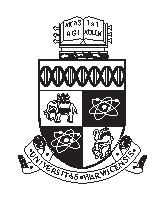
\includegraphics[width=0.4\textwidth]{crest.eps}
	\end{figure}
	\vspace{37mm}
	Cem Yilmaz \\
	\today
	\end{center}
	\end{titlepage}	
	\newpage
	\tableofcontents
	\newpage
\section{Analysis of Algorithms}
\subsection{Classification of a good algorithm}
A good algorithm is one that optimises the following:
\begin{itemize}
	\item Time
	\item Memory
	\item Network bandwidth
	\item Energy consumption
\end{itemize}
However, the main focus in this module will be the running time, in particular, this $O(x)$
\subsection{Running Time}
Running time of an algorithm typical grows with the input size. However, for different inputs of the same size the running time of an algorithm can vary. Then, for an input of fixed size $n$, we have different running times. We can categorise them as the following:
\begin{itemize}
	\item Average case - the typical running time an algorithm requires and is often very difficult to determine
	\item Best case - what is the minimum running time of the algorithm and is generally not useful
	\item Worst case - upper bound on the running time, for any possible input and is more standard to analyse. Our focus is generally this.
\end{itemize}
\subsection{Finding the running time}
\subsubsection{Experimental Analysis}
The first method to use is experimental analysis. For this, we use computer and run simulations. For this, we write a program implementing the algorithm and run the program with inputs of varying size and composition, noting the time needed. However, there are limitations:
\begin{itemize}
	\item It is necessary to implement the algorithm. Sometimes this can be impossible.
	\item Need to make sure that we have considered all kinds of inputs. This sometimes cannot be possible and otherwise it would not be indicative of running time
	\item Different algorithms may run different in different systems due to different features. It can be especially worse for different hardware.
\end{itemize}
\subsubsection{Theoretical Analysis}
The second method is theoretical analysis. For this, we use pen and paper. We use a high-level description of the algorithm instead of an implementation. We then characterise running time as a function of the input size $n$ which takes in account all possible inputs. This would indeed allow us to evaluate the speed of an algorithm independent of the hardware or software environment. A good way to do high level description is to use pseudo-code. We also assume that the algorithm runs in an idealised machine. We assume simple memory hierarchy that is unbounded, infinite precision in arithmetic operations etc. 
\subsection{Random Access Machine (RAM) Model}
It is a simple mode of computation with a singular CPU. It only executes a single program. It also has a bank of memory cells where each cell can hold arbitrarily large positive integers. Every cell gets assigned an ID that allows us to access the information in some \textit{unit time}. In CPU, as learned from CS132, the CPU has the program stored inside. It is also connected to a program counter and registers $R_0,R_1,\ldots$ along with memory cells. It can do basic operations between two numbers stored in the registers, which include but are not limited to:
\begin{itemize}
	\item Addition
	\item Comparison
	\item Fetch an element from the memory
	\item Write an element to the memory
\end{itemize}
However, one thing that categorises and defines RAM as what it is is the fact that \textit{we can access any memory cell in unit times}. 
\subsection{Primitive Operations}
Primitive operations are basic computations that are performed by an algorithm. These take constant time in the RAM model and we count the primitive operations that happen. The assumption is that the number of primitive operations are proportional to the actual running time. Some examples of primitive operations include evaluating an expression, assigning a value, calling a method, indexing into an array etc.
\begin{tcolorbox}[colback=black!3!white,colframe=black!60!white,title=\begin{exmp}Operations in a code \label{Operations in a code}\end{exmp}]
        \begin{lstlisting}[language = Java , caption={Operations} , frame = trBL , firstnumber = last , escapeinside={(*@}{@*)}]
        public static double arrayMax(double[] data) {
		int n = data.length;
		double currentMax = data[0];
		for (int j = 1; j < n; j++)
			if (data[j] > currentMax)
				currentMax=data[j];
		return currentMax;
	}
        \end{lstlisting}
	In particular,
	\begin{itemize}
		\item Step $3$ has $2$ operations
		\item Step $4$ has $2$ operations
		\item Step $5$ has $2n$ operations
		\item Step $6$ has $2n-2$ operations
		\item Step $7$ has $2n-2$ operations and finally
		\item Step $8$ has $1$ operation.
	\end{itemize}
	The code for $arrayMax$ has $6n+1$ as the worst case and $4n+3$ as the best case. Let $T(n)$ be the running time of arrayMax. Then, 
	\begin{align*}
		a(4n+3) \le T(n) \le a(6n+1)
	\end{align*}
Where $a$ is the time to execute a primitive operation.
\end{tcolorbox}
\subsection{Sorting algorithms}
Indeed, the time complexity can be seen clearly in sorting algorithms for times.
\begin{figure}[H]
	\centering
	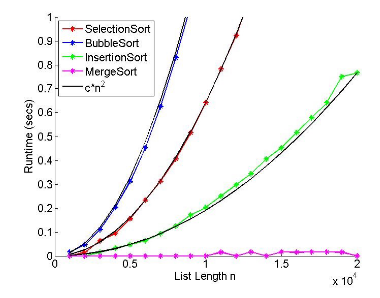
\includegraphics[width=0.6\textwidth]{sorting.png}
	\caption{Complexity of sorting algorithms}
	\label{fig:sorting-png}
\end{figure}
\section{Asymptotic Notation}
\subsection{Big-O notation}
\begin{tcolorbox}[colback=black!3!white,colframe=black!60!white,title=\begin{defn}Big O \label{Big O}\end{defn}]
For two functions $f(n)$ and $g(n)$, we say that $f(n)$ is $O(g(n))$ if there are positive constants $c$ and $n_0$ i.e. $n_0,c\ge 1$ and such that
\begin{align}
	f(n) \le cg(n)
\end{align}
for any $n \ge n_0$ and $n \ge n_0$.
\end{tcolorbox}
\begin{tcolorbox}[colback=black!3!white,colframe=black!60!white,title=\begin{exmp}Example 1 \label{Example 1}\end{exmp}]
        $2n+10$ is in $O(n)$.
                \begin{align}
                2n+10 \le  cn \\
		(c-2)n \ge 10 \\
		n\ge \frac{10}{c-2}
                \end{align}
		We pick $c=3$ and $n_0=10$.
\end{tcolorbox}
\begin{tcolorbox}[colback=black!3!white,colframe=black!60!white,title=\begin{exmp}Example 2 \label{Example 2}\end{exmp}]
        $n^2$ is not $O(n)$
                \begin{align}
                n^2\le cn\\
		n\le c
                \end{align}
		$c$ is a constant and thus this inequality cannot be satisfied.
\end{tcolorbox}
\begin{tcolorbox}[colback=black!3!white,colframe=black!60!white,title=\begin{exmp}Example 3 \label{Example 3}\end{exmp}]
        $7n-2$ is in $O(n)$
                \begin{align}
                7n-2 \le cn
                \end{align}
		Pick $c=7$ and $n_0=1$.
\end{tcolorbox}
\begin{tcolorbox}[colback=black!3!white,colframe=black!60!white,title=\begin{exmp}Example 4 \label{Example 4}\end{exmp}]
        Is is true that $t>0$, $(1+n) ^{t}$ is in $O(n^{t})$
                \begin{align}
			(1+n)^{t} = \sum_{i=0}^{t} {t \choose i} n^{i}
                \end{align}
		However, $t$ is the biggest number therefore it is $O(n^{t})$
\end{tcolorbox}
Thus, the Big-O notation gives an upper bound on the growth rate of a function as $n$ grows towards infinity. We can use the Big-O notation to rank functions according to their growth rate.
\subsubsection{General Rules}
\begin{itemize}
	\item Drop lower order terms
	\item Drop constant terms
	\item Use the smallest possible class of functions
\end{itemize}
\subsection{Relatives of Big-O}
\subsubsection{Big Omega}
\begin{tcolorbox}[colback=black!3!white,colframe=black!60!white,title=\begin{defn}Big Omega \label{Big Omega}\end{defn}]
$f( n)$ is $\Omega(g(n))$ if there is a constant $c > 0$ and an integer constant $c>0$ and an integer constant $n_0\ge 1$ such that for $n\ge n_0$
\begin{align}
f(n) \ge cg(n)
\end{align}
\end{tcolorbox}
\subsubsection{Big Theta}
\begin{tcolorbox}[colback=black!3!white,colframe=black!60!white,title=\begin{defn}Big Theta \label{Big Theta}\end{defn}]
$f(n)$ is $\Theta(g(n))$ if there are constants $c'>0$ and $c'' > 0$ and ann integer constant $n_0 \ge 1$ such that for $n \ge  n_0$
\begin{align}
c'g(n) <f(n) \le c''g(n)
\end{align}

\end{tcolorbox}
\subsubsection{Summary}
\begin{itemize}
	\item Big-$O$ is asymptotically less than or equal to $g(n)$ 
	\item Big-$\Omega$ is asymptotically greater than or equal to $g(n)$ 
	\item Big-$\Theta$ is asymptotically sandwiched between $g(n)$ differing by constant
\end{itemize}
\begin{figure}[H]
    \centering
    \incfig{summaryo}
    \caption{Summary of Big notations graphically}
    \label{fig:summaryo}
\end{figure}
\subsection{Examples}
\begin{tcolorbox}[colback=black!3!white,colframe=black!60!white,title=\begin{exmp}Example 1 \label{Example 1}\end{exmp}]
        $5n^2$ is in $\Omega(n^2)$
                \begin{align}
                5n^2\ge cn^2, \text{ let } c=5, n_0=1
                \end{align}
	$5n^2$ is also $\Omega(n)$
	\begin{align}
		5n^2\ge cn, \text{ let }c=1, n_0=1
	\end{align}
	$5n^2$ is in $O(n^2)$
	\begin{align}
		5n^2 < cn^2, \text{ let } c=6, n_0=1
	\end{align}
	Because $\Omega(n^2)$ and $O(n^2)$, we indeed can say that
	\begin{align}
		\Theta(n^2)
	\end{align} 
\end{tcolorbox}
\begin{tcolorbox}[colback=black!3!white,colframe=black!60!white,title=\begin{exmp}ln N! \label{ln N!}\end{exmp}]
        Prove that $\ln N! = \Theta(N \ln N)$ \\
	There exists $a,b>0$ and integer $N_0 > 0$ such that for any $N \ge  N_0$ we have
                \begin{align}
                a N \ln N \le  \ln N! \le bN \ln N
                \end{align}
		Equivalently, it suffice to prove that
		\begin{align*}
			\ln N! = O(N \ln N) \\
			\ln N! = \Omega (N \ln N)
		\end{align*}
		We begin with proving the upper bound:
		\begin{proof}
			\begin{align*}
				\ln N! = \sum_{i=1}^{N} \ln(i) \\
			\end{align*}
			We also have that $\ln$ is an increasing function, that is for $x>y$ we have $\ln(x)>\ln(y)$ and this implies that for any $1\le i\le N$ we have that $\ln(i) \le  \ln(N)$. Hence, we substitute $\ln(i)$ with $\ln(N)$ in the equation above
			\begin{align*}
				\ln N! = \sum_{i=1}^{N} \ln(i) \le  N \ln(N)
			\end{align*}
			Therefore indeed $\ln N! = O(N \ln N)$
		\end{proof}
		We now prove the lower bound:
		\begin{proof}
			\begin{align*}
				\ln N! = \sum_{i=1}^{N} \ln(i) \ge  \sum_{i=\left\lceil \frac{N}{2} \right\rceil }^{N} \ln(i)
			\end{align*}
			We now observe that $\ln$ is an increasing function, that is for $x>y$ we have $\ln x > \ln y$ which implies that for any $\left\lceil \frac{N}{2} \right\rceil \le i\le N$ we have that $\ln i \ge  \ln(\frac{N}{2})$. Let us now substitute $\ln(i)$ with $\ln(\frac{n}{2})$ in the equation above to obtain
			\begin{align*}
				\ln N! \ge  \sum_{i=\left\lceil \frac{N}{2} \right\rceil }^{N} \ln(i) \ge \left\lceil \frac{N}{2} \right\rceil \ln(\frac{N}{2})
			\end{align*}
			Which indeed shows that $\ln N! = \Omega (N \ln N)$.
		\end{proof}
\end{tcolorbox}

\section{Abstract Data Types (ADT)}
\begin{tcolorbox}[colback=black!3!white,colframe=black!60!white,title=\begin{defn}Abstract Data Type \label{Abstract Data Type}\end{defn}]
An abstract data type is an abstract of a data structure. For an ADT we need to specify
\begin{itemize}
	\item Data stored
	\item Operations on the data
	\item Error conditions associated with operations
\end{itemize}
In abstract data types on what each operation does, but we do not focus on how it does it. In Java, ADT is expressed usually by an interface.
\end{tcolorbox}
\subsection{The Stack ADT}
Intuitively, we can think of a spring-loaded plate dispenser. 
\begin{tcolorbox}[colback=black!3!white,colframe=black!60!white,title=\begin{defn}Stack \label{Stack}\end{defn}]
A stack is a collection of objects that are inserted and removed according to last-in, first out principle. In other words, "LIFO". 
\end{tcolorbox}
\subsubsection{Fundamental Operations}

\begin{itemize}
	\item Push - puts an element at the top of the stack.
	\item Pop - gets the element from the top of the stack.
\end{itemize}
\subsubsection{Main operations}

\begin{itemize}
	\item push(object): inserts an element
	\item pop(): removes and returns the last inserted element. Note that if it is empty we return null, an extreme case.
	\item we recall that insertions and deletions follow the LIFO scheme.
\end{itemize}
\subsubsection{Auxiliary operations}

\begin{itemize}
	\item top(): returns the last inserted element without removing it
	\item size(): returns the number of elements stored
	\item isEmpty() indicates whether no elements are stored
\end{itemize}
\begin{tcolorbox}[colback=black!3!white,colframe=black!60!white,title=\begin{exmp}Operations of a stack \label{Operations of a stack}\end{exmp}]
\begin{figure}[H]
	\centering
	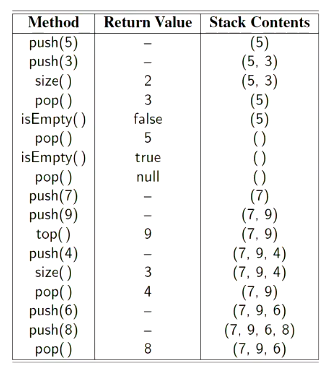
\includegraphics[width=0.4\textwidth]{figures/stack.png}
	\caption{Stack Operations}
	\label{fig:figures-stack-png}
\end{figure}
\end{tcolorbox}
\subsubsection{Application}
The direction applications of stage include page visited history in a web browser, the undo sequence in a text editor and the chain of method calls in the Java Virtual Machine. Another distinct example is to use to match parentheses. \\
The indirect applications include being auxiliary data structure for algorithms and component of other data structures. For example, we could use it to compute spans. For the array $X$, the span $S$ is an array such that $S[i] = \text{the number of consecutive elements}$ $X[j]$ just before $X[i]$ such that $X[j]\le X[i]$.
\subsubsection{Implementation}
The idea involves of adding elements from left to right of the array, with a variable that keeps track of the index of the top element. We would increment and decrement this variable as we push and pop objects into our array. If the array storing the elements suddenly becomes full, then a push operation will throw a FullStackException which is a limitation of the array based implementation. This is not intrinsic to the Stack ADT, and one could do a workaround using ArrayLists. The performance of array based limitation is as follows
\begin{itemize}
	\item Space: It requires space $O(n)$ for storing $n$ elements
	\item Time: Each operation runs in $O(1)$ time
\end{itemize}
Limitations include, but are not limited to
\begin{itemize}
	\item The maximum size of the stack must be defined priori and can't be changed
	\item Trying to push a new element into a full stack causes an implementation-specific exception
\end{itemize}
In terms of performance, it is very good.
\subsection{Queue ADT}
\begin{tcolorbox}[colback=black!3!white,colframe=black!60!white,title=\begin{defn}Queue \label{Queue}\end{defn}]
A queue is a FIFO - first-in, first-out. In comparison to stack which is a LIFO. Insertions are at the rear of the queue and removals are the front of the queue. Priority is given to the one who arrived first. We generally tend to use queues for fairness. It stores arbitrary objects.
\end{tcolorbox}
\subsubsection{Main and fundamental operations}
\begin{itemize}
	\item enqueue(object): inserts the object at the end of the queue
	\item dequeue(): removes and returns the element at the front of the queue. Note that we return null if it is empty, an extreme case
\end{itemize}
\subsubsection{Auxiliary operations}
\begin{itemize}
	\item first(): returns the element at the front without removing it
	\item size(): returns the number of elements stored
	\item isEmpty(): indicates whether no elements are stored
\end{itemize}
\begin{tcolorbox}[colback=black!3!white,colframe=black!60!white,title=\begin{exmp}Operations \label{Operations}\end{exmp}]
        \begin{figure}[H]
        	\centering
        	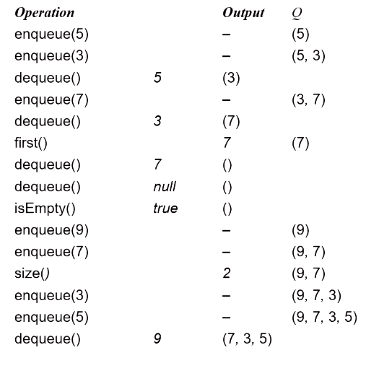
\includegraphics[width=0.5\textwidth]{figures/queue.png}
        	\caption{Operations of queue}
        	\label{fig:figures-queue-png}
        \end{figure}
\end{tcolorbox}
\subsubsection{Application}
Direct applications include waiting lists - queuing theory in mathematics and access to shared resources e.g., printer. For example, round robin schedulers use queues. \\
Indirect applications include auxiliary data structures for algorithms and component of other data structures
\subsubsection{Implementation}
With arrays, the idea is to use an array of size $N$ in a circular fashion. Two variables keep track of the front and the size. $f$ index of the front element and $sz$ number of stored elements. Note that it would be meaning to begin the queue in the middle of the array. When the queue has fewer than $N$ elements, array location $r= (f=sz) \bmod N $ is the first empty slot past the rear of the queue. Note that because we want to be able to use all of the array in circles, it would be viable to implement the modulo $N$ operator. In other words,
\begin{lstlisting}[language = Java , caption={dequeue} , frame = trBL , firstnumber = last , escapeinside={(*@}{@*)}]
if isEmpty() then
	return null
else
	o = Q[f]
	f = (f+1) mod N
	sz = sz-1
	return o
\end{lstlisting}
This is to ensure that overflow of queue can go to the beginning of array instead. In arrays, we cannot add more than $N$ elements due to limitation of arrays. Furthermore, enqueue(o) should throw an exception if the array is full.
\subsubsection{Performances and Limitations}
The performance space is that it requires $O(n)$ for storing $n$ elements \\
The time required for each operation is $O(1)$ time \\
The limitations include the fact that the maximum size of the queue must be defined a priori and cannot be changed. Trying to enqueue a new element into a full queue causes an implementation-specific exception. In terms of performance, we could have not hoped for better as arrays give very quick access to elements.
\subsection{List ADT}
We have seen lists from data structures, namely section \ref{list}. These were data structures and not ADTs. 
\subsubsection{Main, fundamental and auxiliary operations}
\begin{itemize}
	\item set(i,e) - replaces the element at index $i$ with $e$, and returns the old element that was replaced; an error occurs if $i$ is not in range $[0,size\left( \right) -1]$ 
	\item get(i) - returns the element of the list having index $i$; an error condition occurs if $i$ is not in range $[0, size\left(  \right) -1]$
	\item size() - returns the number of elements in the list
	\item isEmpty() - returns a boolean indicating whether the list is empty
	\item add(i,e) - inserts a new element $e$ into the list so that it has index $i$, moving all subsequent elements one index later in the list. An error condition occurs if $i$ is not in range $[0,size\left(  \right) ]$.
	\item remove(i) - removes and returns the element at index $i$, moving all subsequence elements on index earlier in the list; an error condition occurs if $i$ is not in the range $[0,size\left(  \right) -1]$.
\end{itemize}
\begin{figure}[H]
	\centering
	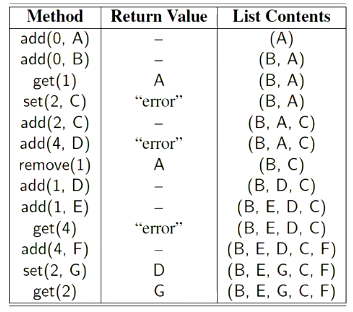
\includegraphics[width=0.45\textwidth]{figures/listadt.png}
	\caption{List Operations Example}
	\label{fig:figures-listadt-png}
\end{figure}
\subsubsection{Implementation}
A natural choice for implementing the list ADT is to use an array, $A$. The idea is that $A[i]$ stores a reference to the element with index $i$ in the list. The methods get(i) and set(i,e) are easy to implement by accessing  $A[i]$. \\
We insert element by using the operation add(i,o). The challenge is that we need to make room for the new element, meaning that we are shifting forward the $n-i$ elements $A[i],\ldots,A[n-1]$. The worst case corresponds to having $i=0$, if there are $n$ elements already in the list then we require to shift it by $n$. With removing elements, the challenge is to fill the hole left by the removed element. Shift backward the $n-i-1$ elements $A[i+1],\ldots,A[n-1]$, which means that at the worst we obtain $n$ shifts.
\subsubsection{Performance}
Suppose that we have a list $L$ with size $n$, there are $n$ elements in $L$. The space required for $L$ is $O(n)$, assuming that each reference object requires $O(1)$. Add and remove require in worst $O(n)$ operations. The limitations is that we cannot store more elements than the size of the array. If the array is full, the add operation throws an exception.
\subsection{ArrayList ADT}
In addition to the list ADT,
If the array is full, instead of throwing an exception for push(o), let us
\begin{enumerate}
	\item replace the array with a larger one
	\item insert the new element
\end{enumerate}
\begin{lstlisting}[language = Java , caption={push} , frame = trBL , firstnumber = last , escapeinside={(*@}{@*)}]
if size=S.length then
tmp = new array of size ...
for i = 0 to S.length-1
	tmp[i] = S[i]
S = tmp
S[n] = o
\end{lstlisting}
The question stands, how big should the new array be:
\begin{itemize}
	\item Incremental strategy - increase the size by some constant $c$ 
	\item Doubling strategy - double the size
\end{itemize}
Let us measure the comparison of the two strategies. Consider $T(n)$ the elementary operations needed to perform a series of $n$ push operations. Each one of the incremental and double strategy gives a rise to a different $T(n)$. We will compare the strategies in terms of corresponding quantities $T(n)$ Assume
\begin{itemize}
	\item We start with an empty list
	\item The initial size of the array is $1$
\end{itemize}
We call amortised time of a push operation the "average time" each push operation require i.e., $\frac{T(n)}{n}$.
\subsubsection{Incremental strategy - analysis}
Over $n$ push operations we place the array $k = \left\lfloor \frac{n}{c} \right\rfloor$ times, where $c>0$ is a constant independent of $n$. The total time $T(n)$ of a series of $n$ push operations is proportional to 
\begin{align*}
	c+2c+3c+4c+\ldots+kc = \\
	c(1+2+3+\ldots+k) = \\
	\frac{c}{2}k(k+1)
\end{align*}
Note that the reason for increase is because we keep adding new elements and when creating the new array we require to create a bigger array and transfer more data each time, and this is incremented by $c$ each time for an array of size $c$. \\
Since $c$ is a constant, $T(n) = \Omega(k^2) = \Omega(n^2)$.
The amortised time of a push operation is $\Omega(n)$. The above analysis gives us an "asymptotic lower bound" for the amortised time.
\subsubsection{Doubling strategy - analysis}
Over $n$ pushes operations we replace the array $k = \log_2 n$ times. The total time $T(n)$ of a series of $n$ push operations is proportional to
\begin{align*}
	1+2+4+8+\ldots+2^{k} = 2^{k+1}-1 = 2n-1
\end{align*}
Therefore $T(n)$ is $O(n)$, the amortised time of a push operation is then on average $O(1)$.
\subsubsection{Remarks on strategies}
Although amortised time for doubling strategy is only $O(1)$, we need to realise that the doubling strategy is not so economical in the use of space. With the doubling strategy we win in time/operation but we lose in space usage.
\subsection{Positional List ADT}
\subsubsection{Main, fundamental and auxiliary operations}
\begin{itemize}
	\item first(): returns the position of the first element of $L$ or null if empty
	\item last(): returns the position of the last element of $L$ or null if empty
	\item before(p): returns the position of $L$ immediately before position $p$ (or null if $p$ is the last position)
	\item after(p): returns the position of $L$ immediately after position $p$ (or null if $p$ is the last position)
	\item isEmpty(): returns true if list $L$ does not contain any elements
	\item size(): returns the number of elements in list $L$
	\item addFirst(e): Inserts a new element $e$ at the front of the list, returning the position of the new element
	\item addLast(e): Inserts a new element $e$ at the back of the list, returning the position of the new element
	\item addBefore(p,e): Inserts a new element $e$ in the list, just before position $p $, returning the position of the new element
	\item addAfter(p,e): Inserts a new element $e$ in the list, just after position $p$, returning the position of the new element
	\item set(p,e): replaces the element at the position  $p$ with element $e$, returning the element formerly position $p$.
	\item remove(p): removes and returns the element at position $p$ in the list, invalidating the position.
\end{itemize}
\begin{figure}[H]
	\centering
	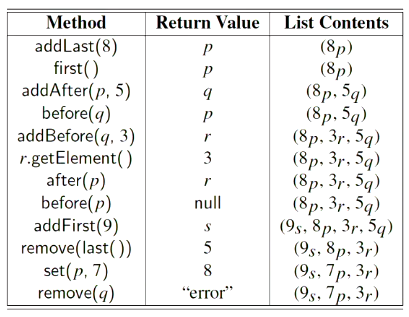
\includegraphics[width=0.45\textwidth]{figures/positional.png}
	\caption{Positional List Operations}
	\label{fig:figures-positional-png}
\end{figure}
A natural way to implement positional list ADT is by the doubly linked list.
\subsection{Maps ADT}
\begin{tcolorbox}[colback=black!3!white,colframe=black!60!white,title=\begin{defn}Maps \label{Maps}\end{defn}]
Maps are searchable collection of key-value entries where each entry is $(key,value)$
\end{tcolorbox}
Intuitively, a map $M$ supports the \textbf{abstraction} of using keys as indices with a syntax like $M[k]$, very similar to that of an array. As a map with $n$ items uses keys that are known to be integers in a range from $0$ to $N-1$, for some $N \ge n$ we can just use an array..
\subsubsection{Main, fundamental and auxiliary operations}
\begin{itemize}
	\item get(k): if the map $M$ has an entry with key $k$, return its associated value; else, return null
	\item put(k,v): insert entry $(k,v)$ into the map $M$ ; if the key $k$ is not already in $M$, then return null; else, return old associated value with $k$.
	\item remove(k): if the map $M$ has an entry with key $k$, remove it from $M$ and return its associated value; else, return null
	\item size(), isEmpty()
	\item entrySet(): return an iterable collection of the entries in $M$ 
	\item keySet(): return an iterable collection of the keys in $M$
	\item values(): return an iterator of the values in $M$
\end{itemize}
\begin{tcolorbox}[colback=black!3!white,colframe=black!60!white,title=\begin{exmp}Operations example \label{Operations example}\end{exmp}]
\begin{figure}[H]
	\centering
	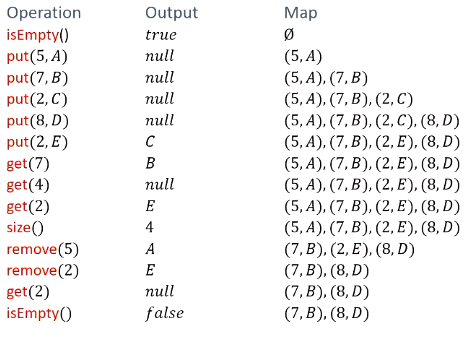
\includegraphics[width=0.5\textwidth]{figures/map.png}
	\caption{Map operations example}
	\label{fig:figures-map-png}
\end{figure}
\end{tcolorbox}
Note that multiple entries with the same key are not allowed.
\subsubsection{Implementation}
Our implementation will be done using an unsorted list this time. We store the items of the map in a list $S$ (based on a doubly linked list) in an arbitrary order. For example, to implement get(k) we would
\begin{lstlisting}[language = Java , caption={get(k)} , frame = trBL , firstnumber = last , escapeinside={(*@}{@*)}]
algorithm get(k):
B = S.positions()
while B.hasNext() do
	p = B.next()
	if p.element().getKey() == k then
		return p.element().getValue()
return null
\end{lstlisting}
and for put
\begin{lstlisting}[language = Java , caption={put(k,v)} , frame = trBL , firstnumber = last , escapeinside={(*@}{@*)}]
B = S.positions()
while B.hasNext() do
	p = B.next()
	if p.element().getKey() == k then
		t = p.element().getValue()
		S.set(p,(k,v))
		return t //return the old value
S.addLast((k,v))
size = size+1 // increase size as we are adding
return null //no previous entry was found
\end{lstlisting}
and for remove
\begin{lstlisting}[language = Java , caption={remove(k)} , frame = trBL , firstnumber = last , escapeinside={(*@}{@*)}]
B = S.positions()
while B.hasNext() do
	p = B.next()
	if p.element().getKey() == k then
		t = p.element().getValue()
		S.remove(p)
		size--
		return t
return null
\end{lstlisting}
\subsubsection{Applications}
Address book and student-record databases.
\subsubsection{Performance}
\begin{itemize}
	\item put requires $O(n)$ operations in the worst case as it may need to traverse the entire sequence to check whether the new element already exists. 
	\item get and remove for similar reasons also require $O(n)$ times, as we require to search to see if the $k$ exists.
	\item The performance in general is poor, we would like to have $O(\log n)$ or $O(1)$ operations, and the unsorted list implementation is effectively only for maps of small size. For example, sort would be able to give us a method of implementing binary search to search for the $K$.
\end{itemize}
\subsubsection{Hashing}
To generalise our previous question about having non-integer keys we can use something called the hashing function
\begin{tcolorbox}[colback=black!3!white,colframe=black!60!white,title=\begin{defn}Hashing Function \label{Hashing Function}\end{defn}]
A hash function generates a map of data of arbitrary size a fix size value. This generates keys for any input key. It begins with hash code:
\begin{align*}
	h_1:& \text{keys} \to \text{integers} \\
	h_2:&\text{integrs}\to [0,N-1]
\end{align*}
The hash code is applied first and the compression function is applied next to the result 
\end{tcolorbox}
\begin{tcolorbox}[colback=black!3!white,colframe=black!60!white,title=\begin{exmp}Hash Function Example \label{Hash Function Example}\end{exmp}]
        The $h(x)$ defined as
                \begin{align}
                h(x) = x   \bmod N  
                \end{align}
		is a hash function for integer keys
\end{tcolorbox}
\begin{tcolorbox}[colback=black!3!white,colframe=black!60!white,title=\begin{defn}Hash Table \label{Hash Table}\end{defn}]
A has table for a given key type consists of 
\begin{itemize}
	\item hash function $h(x)$
	\item array, of size $N$ called table
\end{itemize}
When implementing a map with hash table, the goal is to store item $(k,o)$ at the index $i = h(k)$.
\end{tcolorbox}
For example, entries with (SSN, Name), say we use an array data of length $10000$ and store entry $(k,v)$ in cell data[i] where $i = \text{ last } 4 \text{ digits of }k$. Then,
\begin{align*}
	h(025-612-0001)=0001
\end{align*}
\begin{tcolorbox}[colback=black!3!white,colframe=black!60!white,title=\begin{defn}Collision \label{Collision}\end{defn}]
Suppose for our hash function above for SSN, what happens if there are distinct datas that generate the same hash index? In such case, the answer is not trivial with no clear solution. Note that collision is bound to happen because by nature hashing is the idea of mapping an arbitrarily large size data to a fixed data size.
\end{tcolorbox}
\begin{tcolorbox}[colback=black!3!white,colframe=black!60!white,title=\begin{defn}Horner's Rule \label{Horner's Rule}\end{defn}]
Polynomial $p(z)$ can be evaluated in $O(n)$ time
\begin{align}
p_0(z) = a_{n-1}\\
p_i(z) = a_{n-i-1}+zp_{i-1}(z)
\end{align}
for $i=1,2,\ldots,n-1$ we have $p(z)=p_{n-1}(z)$. That is, each new $p$ is computed from the previously one in $O(1)$ time
\end{tcolorbox}
\subsubsection{Methods of reducing collision (Collision Handling)}
\begin{itemize}
	\item Separate chaining - let each cell in the table point to a map of entries, i.e., multiple instances in one cell. Separate chaining is simple, but requires additional memory outside the table
	\item Linear probing - reduce collision through open addressing. The colliding item is placed in a different cell of the table. It handles collisions by placing the colliding item in the next available table cell. This can cause lumps of collided elements
	\item Double hashing - uses two hash functions $h$ and $f$. If cell $h(k)$ is already occupied, it tries sequentially another cell. The secondary has function $f(k)$ cannot have zero values. The table size $N$ must be a prime to allowing probing of all the cells. It generalises linear probing. E.g., $h(k) + i f(k)  \bmod N $. In some sense, the secondary function allows for lumps not to be created because of the second function.
\end{itemize}
\subsubsection{Performance}
Worst case, searches, insertions and removals on a hash table take $O(N)$ time. The worst case scenario occurs when all the keys inserted into the map collide. In practice, we like to deal the hush function as generating random hash values. Worst case analysis is not the optimal approach. We measure this by load factor
\begin{align*}
	\alpha = \frac{n}{N}
\end{align*}
affects the performance of a hash table. $n$ is the number of elements in table and $N$ is the size of the table. Each has value we generate has probability $\alpha$ of creating collision. The "expected number" of problems for an insertion with open addressing is
\begin{align*}
	\frac{1}{a-\alpha}
\end{align*}
In practice, hashing is very fast provided the load factor is \textit{not} close to $1 $.
\subsection{Priority Queue ADT}
\subsubsection{Main, fundamental and auxiliary operators}
A priority queue stores a collection of entries where each entry is a pair (key, value)
\begin{itemize}
	\item insert(k,v)
	\item removeMin() removes and returns the entry with smallest key, or null if the priority queue is empty
\end{itemize}
Auxiliary methods include
\begin{itemize}
	\item min()
	\item size()
	\item isEmpty()
\end{itemize}
\subsubsection{Implementation}
We can implement priority queue using an unsorted list. Insertion takes $O(1)$ time, removeMin and min takes $O(n)$ time since we have to traverse the entire sequence to find the smallest key.
\subsection{Entry ADT}
\subsubsection{Main, fundamental and auxiliary operators}
An entry in PQ a key-value pair. It stores entries to allow for efficient insertion and removal based on keys. Methods for entry include:
\begin{itemize}
	\item getKey(): returns the key for the entry
	\item getValue: returns the value in this entry
\end{itemize}

\subsection{Tree ADT}
\subsubsection{Main, fundamental and auxiliary operators}
We use positions to abstract nodes. Generic methods:
\begin{itemize}
	\item size()
	\item isEmpty()
	\item iterator()
	\item positions()
\end{itemize}
Accessors methods include
\begin{itemize}
	\item root()
	\item parent()
	\item children(p)
	\item numChildren(p)
\end{itemize}
\subsubsection{Traversal}
Preorder traversal is a method of going through all nodes of a tree in a systematic manner. In a preorder traversal, a node is printed before its descendants
\subsection{Set ADT}
\subsubsection{Main, fundamental and auxiliary operators}
\begin{itemize}
	\item add(e): Adds the element e to S if not already present
	\item remove(e): Removes the element e from S if present
	\item contains(e): Returns whether e is an element of S
	\item iterator(): Returns an iterator of elements of S
\end{itemize}
For which it is also usually implemented with traditional mathematical set operations i.e., $S \cap T$, $S \cup T$, $ S - T$.
Auxiliary methods include:
\begin{itemize}
	\item addAll(T): Updates S to include all elements of set T.
	\item retainAll(T): Updates S so that it only keeps those elements that are also elements of the set T.
	\item removeAll(T): Updates S by removing any of its elements that also occur in the set T.
\end{itemize}
\subsubsection{Implementation}
We can implement a set with a list. Elements are stored according to some canonical ordering with space $O(n)$. Things such as union can be implemented using GenericMerge \ref{gm}. For example, let
\begin{align*}
	A = \{ 5,7,11,12,15\} & B = \{ 3,5,14,15,22,27\}
\end{align*}
Then, our Generic Merge would be as follows:
\begin{enumerate}
	\item Compare $5$ and $3$.  Notice $3<5$, then, remove $3$ from $B$ and add it to $S$.
	\item Compare $5$ and $5$. Notice $5=5$, then, remove both $5$ from $A$ and $B$ and add it to $S$.
	\item Compare $11$ and $14$. Notice $11<14$, then, remove $11$ from $A$ and add it to $S$.
	\item $\ldots$ 
	\item We then add the last elements of the bigger set.
\end{enumerate}
Note that these run in linear time i.e., $O(n_A + n_B)$ time, provided the auxiliary methods run in $O(1)$ time.
\section{Data Structures}

\subsection{Arrays}
\begin{tcolorbox}[colback=black!3!white,colframe=black!60!white,title=\begin{defn}Array \label{Array}\end{defn}]
An array is a sequences collection of variables of thesame type. Each variable, or cell, in an array has an index, which uniquely refers to the value stored in that cell.

A value stored in an array is often called an element.

The length of an array determines the maximum number of elements that can be stored.
\end{tcolorbox}
\subsubsection{Strengths}
\begin{itemize}
	\item We assume that we can access each cell $k$ in $O(1)$ time.
	\item You can write or read once accessed.
	\item Access time is very fast $O(1)$.
\end{itemize}
\subsubsection{Limitations}
\begin{itemize}
	\item We cannot change the length of an array
\end{itemize}
\subsubsection{Declaring arrays in Java}
Assignment to a literal form when initially declaring the array
\begin{lstlisting}[language = Java , caption={Array} , frame = trBL , firstnumber = last , escapeinside={(*@}{@*)}]
elementType[] arrayName = { v0, v1, ..., vn-1}
\end{lstlisting}
elementType : any Java base type, or class name

arrayName : any valid Java identifier

Remark : the initial values must be of the same type as the array.

We also use the new operator to declare arrays because it is not an instance of a class. That is,
\begin{lstlisting}[language = Java , caption={Declaring array} , frame = trBL , firstnumber = last , escapeinside={(*@}{@*)}]
new elementType[length]
\end{lstlisting}
The new operator returns a reference to the new array. This is assigned to the array variable measurements.
\begin{lstlisting}[language = Java , caption={Example} , frame = trBL , firstnumber = last , escapeinside={(*@}{@*)}]
double [] measurements = new double [1000]
\end{lstlisting}
\subsubsection{Examples}
A array can store primitive elements, such as characters. E.g.
\begin{table}[H]
	\centering
	\caption{Primitive element array}
	\label{tab:label}
	\begin{tabular}{|c|c|c|c|c|c|}
	\hline
	S & A  & M  & P  & L & E  \\
	\hline
	0 & 1 & 2 & 3 & 4 & 5 \\
	\hline
	\end{tabular}
\end{table}
...or pointer to references to objects. For example, the first cell can refer to the pointer of the word "Joseph" and the second can refer to the pointer of "Helen" etc.
\subsubsection{Adding an entry}
To add an entry $e$ into array board at $i$ we need to make room. We shift each $n-i \mapsto n-i+1$. This is $O(n-i)$.
\subsubsection{Concluding Remarks}
\begin{itemize}
	\item Read/write any element in $O(1)$ time
	\item The capacity does not change
	\item Shifting $k$ elements requires $O(k)$ time
	\item Very easy to work with
	\item We are going to use arrays a lot when we implement
\end{itemize}
\subsection{Linked Lists \label{list}}
\subsubsection{Singly Linked List}
\begin{tcolorbox}[colback=black!3!white,colframe=black!60!white,title=\begin{defn}Singly Linked List \label{Singly Linked List}\end{defn}]
A singly linked list is a concrete data of structure consisting fro a sequence of nodes, starting from a head pointer.
\end{tcolorbox}
Each node stores element and a link to the next node. However, nodes do not have information on previous nodes. The first node is usually called head, and the last is called tail. However, if the node is tail, then the next link is NULL. However, to access $k$-th element in the node, we would then require to repeat getting node $k-1$ times. This is called pointer hopping.
\begin{figure}[H]
	\centering
	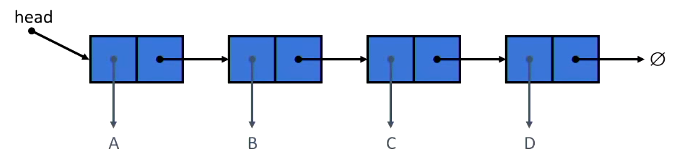
\includegraphics[width=0.8\textwidth]{figures/singlelinkedlist.png}
	\caption{Singly Linked List}
	\label{fig:figures-singlelinkedlist-png}
\end{figure}
Note that the element after the last node is set to null.
\subsubsection{Time required for Singly Linked List}
Our assumption is that CurrentNode.getNext() requires $O(1)$ time. In order to access $k$-th element, we need $O(k)$ time.
\subsubsection{Insertion of head}
To insert a head:
\begin{itemize}
	\item Allocate a new node
	\item Insert a new element
	\item New node points to old head
	\item Update head to point new node
\end{itemize}
This requires $O(1)$ time to insert a new head, as all of the steps taken are a constant. 
\subsubsection{Insertion of tail}
To insert a tail:
\begin{itemize}
	\item Allocate a new node
	\item Insert a new element
	\item New node points to null
	\item Have old last node point to new node
	\item Update tail to point to new node
\end{itemize}
This also requires $O(1)$ time, as all of the steps taken are a constant.
\subsubsection{Remarks}
There is no bound to the maximum number of elements we can store in a list. Therefore, as opposed to the array where the capacity is fixed, i.e., does not changed, the list is more flexible. Furthermore, the operation for insert is only $O(1)$ same as arrays. However, note that when inserting data in the middle of a linked list, we would require to search for the previous node which takes $O(k)$ time. The insertion itself, however, is $O(1)$.
\subsubsection{Removing from head}
Removing from the head requires
\begin{itemize}
	\item Update head to point to next node in the list
	\item Garbage collector reclaims the former first node
\end{itemize}
This therefore requires $O(1)$ time.
\subsubsection{Removing from tail}
Removing from tail requires
\begin{itemize}
	\item Update tail to null
	\item We need to access the node that shows towards the tail
\end{itemize}
This operation therefore requires $\Theta(k)$ time, making it an expensive operation as we required to gain access to the tail.
\subsubsection{Doubly linked list}
In a doubly linked list, nodes store an element, link to the previous node and a link to the next node.
\subsubsection{Insertions in a doubly linked list}
Similar to singly linked list, we would now also have to update pointers for previous pointers also. 
\subsubsection{Deletion in a doubly linked list}
Deletion of a pointer in the trailer is now $O(1)$ since we can simply access it from the last node. Everything else stays the same.
\subsubsection{List VS Array}
Access time for $k$ th element:
\begin{itemize}
	\item Array requires $O(1) $
	\item Singly liked list requires time $O(k)$ 
	\item Doubly linked list requires time $min\{O(k),O(n-k)\}$, we can traverse it from the back
\end{itemize}
For capacity
\begin{itemize}
	\item Array does not change capacity
	\item In both kinds of lists we can add and remove element with no restriction
	\item The time we need to add or remove an element in the list depends n the time we need to access the position of the list that we need to add or remove the element.
	\item Addition and removal is faster when ti is applied to the first or last element and takes $O(1)$ time.
\end{itemize}
\section{Java Fundamentals}
\subsection{Recursion}

\subsubsection{Factorial}
The recursive definition for factorial is:
\begin{align*} f(n) = 
	\begin{cases}
		1 &\text{ if } n = 0 \\
		n \cdot f (n-1) &\text{ otherwise}
	\end{cases} 
\end{align*}
\begin{lstlisting}[language = Java , caption={Factorial in Java} , frame = trBL , firstnumber = last , escapeinside={(*@}{@*)}]
public static int factorial(int n) throws IllegalArgumentException {
if (n < 0)
	throw new IllegalArgumentException();
else if (n == 0)
	return 1;
else
	return n * factorial(n-1);
}
\end{lstlisting}
\subsubsection{Content of a recursive method}
There is always a base case. For example, for factorial we have the base case as $n=0$. \\
There is also always also recursive calls. Each recursive call should be defined so that it makes progress to a base case.
\subsubsection{Linear recursion}
Recur once - perform a single recursive call. This step may have a test that decides which of several possible recursive calls to make, but it should ultimately make just one of these calls. The term "linear recursion" reflects the structure of the trace and not the asymptotic analysis. 
\subsubsection{Binary recursion}
Binary recursion performs two recursive calls. 
\begin{tcolorbox}[colback=black!3!white,colframe=black!60!white,title=\begin{exmp}Integer array A adder \label{Integer array A adder}\end{exmp}]
        Algorithm: $binarySum(A,i,n)$ \\
	Input: Array of integers $A$, where Integers $0\le i, n<A.length()$. \\
	Output: Sum of the $n$ entries in $A$ starting at index $i$.\\
	if $n=1$ then\\
		return $A[i]$\\
	else
		return $binarySum(A,i,\left\lfloor \frac{n}{2} \right\rfloor) + binarySum(A,i+\left\lfloor \frac{n}{2} \right\rfloor, \left\lfloor \frac{n}{2} \right\rfloor)$ \\
		This in fact creates a binary tree.
\end{tcolorbox}
\begin{tcolorbox}[colback=black!3!white,colframe=black!60!white,title=\begin{exmp}Fibonacci \label{Fibonacci}\end{exmp}]
        Fibonacci numbers is an infinite sequence of integers $0,1,1,2,3,5,8,13,21,34,55,89,\ldots$. There is a nice recursive definition for which
                \begin{align}
                F_i = F_{i-1}+F_{i-2}
                \end{align}
		with boundary case corresponding to $F_0=0$ and $F_1=1$.
		Then, we cold write
		\begin{lstlisting}[language = Java , caption={Fibonacci} , frame = trBL , firstnumber = last , escapeinside={(*@}{@*)}]
		if (n=1 || n=0)
			return n;
		else
			return binaryFib(n-1)+binaryFib(n-2)
		\end{lstlisting}
		Everything in the operation is $O(1)$, however, let us denote $n_k$ be the number of recursive calls by $BinaryFib(k)$. It seems that $n_k$ doubles every other time. This means $n_k > 2^{\frac{k}{2}}$. The running time, is then, exponential in $k$. Exponential algorithms are generally not good. This can be instead turned into linear recursion
	
\end{tcolorbox}
\subsubsection{Multiple recursion}
Here is a summation puzzle, where
\begin{enumerate}
	\item $pot+pan = bib$ 
	\item $dog+cat=pig$ 
	\item $boy+girl=baby$
\end{enumerate}
Our task is to assign a unique digit $0,1,\ldots,9$ to each letter in the equation in order to make the equation true. There are $n^{m}$ solutions where $n$ is the number of digits and $m$ is the number of letters.
\begin{tcolorbox}[colback=black!3!white,colframe=black!60!white,title=\begin{exmp}Multiple recursion solution \label{Multiple recursion solution}\end{exmp}]
        Algorithm: $PuzzleSolve(k,S,U)$. \\
	Input: $\text{integer} 0<k, \text{set of elements }S,U $ \\
	Output: enumeration of all $k$-element extensions to $S$ using elements in $U$, without repetitions \\
	For example, say $k=1$ and $U = \{3,4,5\}$ and $S = (1,2)$. Then the algorithm generates the sequences $(1,2,3),(1,2,4),(1,2,5)$ If we had $k=2$, then we need to complete $(1,2,*,*)$ using $\{3,4,5\}$ without repeating numbers. We can see that if we add $k$, the number of solutions double. 
	\begin{lstlisting}[language = Java , caption={PuzzleSolve} , frame = trBL , firstnumber = last , escapeinside={(*@}{@*)}]
	for each element e in U do
	add e to the end of S
	if k = 1, then
		test whether S is a configuation that solves the puzzle
		if S solve sthe puzzle then
		return "Solution found:" S
	else
		PuzzleSolve(k-1,S,U)
	add e back to U
	remove e from the end of S
	\end{lstlisting}
	\begin{figure}[H]
		\centering
		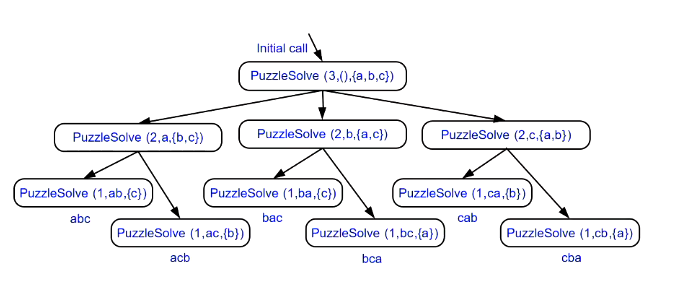
\includegraphics[width=0.8\textwidth]{figures/solver.png}
		\caption{Puzzle Solver Visualisation}
		\label{fig:figures-solver-png}
	\end{figure}
\end{tcolorbox}
\subsection{Iterators}
Sometimes for abstract data structures we require to iterate over elements of an array. For example, if we want to copy array $A$ onto some array $B$, then we would
\begin{lstlisting}[language = Java , caption={Array Copy} , frame = trBL , firstnumber = last , escapeinside={(*@}{@*)}]
for (i=0; i<A.length; i++) {
	B[i] = A[i]
}
\end{lstlisting}
\begin{tcolorbox}[colback=black!3!white,colframe=black!60!white,title=\begin{defn}Iterator \label{Iterator}\end{defn}]
Iterators are software design pattern which abstracts the process of scanning through a sequence one element at a time. A good example is a for-each loop, which is an implicit iterator.
\end{tcolorbox}
However, this does not allow us to iterate over the elements of a positional list. For this we use a construction called iterator. It is common in OOP languages. We would write this as
\begin{lstlisting}[language = Java , caption={Iterator} , frame = trBL , firstnumber = last , escapeinside={(*@}{@*)}]
Iterator<String> iter;
while (iter.hasNext()){
	String value = iter.next();
	System.out.println(value);
}
\end{lstlisting}
The commands
\begin{itemize}
	\item hasNext(): returns true if there is at least one additional element in the sequence and false otherwise
	\item next(): Returns the next element in the sequence
\end{itemize}
Java defines a parameterised interface named Iterable. Iterator() returns an iterator of the elements in the collection. An instance of a typical collection class in Java, such as an ArrayList, is iterable. It produces an iterator for its collection as the return value of iterator(). Each call to iterator() returns a new iterator instance. It also allows for multiple and simultaneous traversals of a collection. for each loops iterate over the element by the syntax
\begin{lstlisting}[language = Java , caption={For each loop} , frame = trBL , firstnumber = last , escapeinside={(*@}{@*)}]
for (ElementType variable : collection) {
	loopBody
}
\end{lstlisting}
\section{Sorting}
\subsection{Sorting Problem}
We are given a sequence of unordered elements, for example
\begin{align*}
	[3,6,2,7,8,10,22,9]
\end{align*}
We want to put the elements into a non decreasing order, i.e., from smaller to larger, in particular we want
\begin{align*}
	[2,3,6,7,8,9,10,22]
\end{align*}
\subsection{Generic Merge \label{gm}}
Generalised merge of two sorted lists $A$ and $B$. We will use the template method $genericMerge$ with auxiliary methods aIsLess, bIsLess and bothAreEqual.
 \begin{lstlisting}[language = Psuedo , caption={Psuedo code for generic merge} , frame = trBL , firstnumber = last , escapeinside={(*@}{@*)}]
algorithm genericMerge(A,B)
	S <- empty sequence
	while not(A.isEmpty) and not(B.isEmpty())
		a <- A.first().element(); b <- B.first().element()
		if a < b
			aIsLess(a,S); A.remove(A.first())
	2222222222	else if b < a
			bIsLess (b,S); B.remove(B.first())
		else 
			bothAreEqual(a,b,S)
			A.remove(A.first()); B.remove(B.first())
	while not(A.isEmpty())
		aIsLess(a,S); A.remove(A.first())
	while not(B.isEmpty())
		bIsLess(b,S); B.remove(B.first())
	return S
\end{lstlisting}
\subsection{Divide and Conquer}
Divide and conquer is a general algorithm design paradigm that:
\begin{itemize}
	\item Divide: Divide the input $S$ into two disjoint subsets $S_1$ and $S_2$.
	\item Recur: Solve the sub problems associated with $S_1$ and $S_2$.
	\item Conquer: Combine the solutions for $S_1$ and $S_2$ into a solution for $S$.
\end{itemize}
The base case for the recursion are sub problems of size $0$ or $1$.
\subsection{Merge Sort}
\subsubsection{Method}

Merge sort utilises divide and conquer. The input is a sequence $S$ with $n$ elements. There are $3$ steps:
\begin{enumerate}
	\item Divide: partition $S$ into two sequences $S_1$ and $S_2$ of about $\frac{n}{2}$ elements each
	\item Recur: recursively sort $S_1$ and $S_2$ 
	\item Conquer: merge $S_1 $ and $S_2$ into a unique sorted sequence
\end{enumerate}
\begin{lstlisting}[language = Pseudo , caption={mergeSort(S)} , frame = trBL , firstnumber = last , escapeinside={(*@}{@*)}]
input: sequence S of n elements
output: sequence S sorted
if S.size() > 1
	(S1,S2) <- partition(S, n/2)
	mergeSort(S1)
	mergeSort(S2)
	S <- merge(S1,S2)	
\end{lstlisting}
The clever part of this sort comes from its merge function, which is defined as the generic merge \ref{gm}. Note that merging two sorted sequences, each with $\frac{n}{2}$ elements and implemented by means of a doubly linked list, takes $O(n)$ time. 
\subsubsection{Running time}
The worst case amount of comparisons is $O(n_A+n_B)$ when one of the lists size is not the same as the other and the best case is $min(n_A,n_B)$. The best case occurs when one of the sets is strictly bigger/smaller than every element in the other set.  \\
The height $h$ of merge-sort tree is $O(\log n)$
\begin{proof}
	The overall amount of work done at the nodes of depth $i$ is $O(n)$. We partition and merge $2^{i}$ and sequences of size $\frac{n}{2^{i}}$. We make $2^{i+1}$ recursive calls. Thus the total running time of merge-sort is $O(n \log n)$. In otherwords, $O(\log n) \times  O(n) = O(n \log n)$. That is, it is the work done at each depth of node times the height. \\
	Remember that the last depth of the tree is actually the height $h$. Then, we know for the number of nodes $n$ 
	\begin{align*}
		1+2+2^{2}+\ldots+2^{h-1} &= \frac{1-2^{h}}{-1} \text{ Geometric Sequence formula} \\
		n &= 2^{h}-1 \\
		\log_{2}(n+1) &= h
	\end{align*}
\end{proof}
\subsection{Sorting with Priority Queue}
\begin{enumerate}
	\item Insert the elements one by one into the PQ with a series of insert()
	\item Remove the elements in sorted order with a series of removeMin()
\end{enumerate}
The running time of this sorting method depends on the priority queue implementation. For selection sort, we use the variation of PQ sort where the priority queue uses an unsorted sequence. Selection sort takes
\begin{align*}
	O(n) + O(n-1) + \ldots + O(1) = O(n^2)
\end{align*}
Selection sort takes $O(n^2)$. Similarly, there is insertion sort. The variation of PQ sort where the priority queue is implemented with a sorted sequence, the running time of insert-sort is
$O(1)+O(2) + \ldots O(n) = O(n^2)$ due to insertion. removeMin then would take $O(n)$.
\subsection{Quicksort}
\subsubsection{Method}
Quicksort is a randomised sorting algorithm based on the divide-and-conquer paradigm:
\begin{enumerate}
	\item Divide: pick a random element $x$ (called pivot) and partition $S$ into
		\begin{itemize}
			\item $L$ elements less than $x$ 
			\item $E$ elements equal $x$ 
			\item $G$ elements greater than $x$
		\end{itemize}
	\item Recur: sort $L$ and $G$ 
	\item Conquer: join $L,E$ and $G$
\end{enumerate}
\begin{lstlisting}[language = Psuedo , caption={Partition} , frame = trBL , firstnumber = last , escapeinside={(*@}{@*)}]
input: sequence S. position p of pivot
output: subsequences L,E,G of the elemenets of S less than, equal to, or greater than the pivor respectively
L,E,G <- empty sequences
x <- S.remove(p)
while not(S.isEmpty())
	y <- S.remove(S.first())
	if y < x
		L.addLast(y)
	else if y == x
		E.addLast(y)
	else
		G.addLast(y)
	return L,E,G
\end{lstlisting}
We partition an input sequence $S$ by removing in turn each element $y$ from $S$ and insert $y$ into $L$, $E$ or $G$, depending on the result of the comparison with the pivot $x$.
\subsubsection{Running time}
Each insertion, removal and comparison takes $O(1)$ and thus the partition step of quick-sort takes $O(n)$ time. Worst case for quick-sort occurs when the pivot is the unique minimum or the unique maximum element. One of $L$ and $G$ has size $n-1$ and the other has size $0$. The running time is proportional to the sum, then,
\begin{align*}
	&n + (n-1) + \ldots + 2 + 1
	=& O(n^2)
\end{align*}
The expected running time, that is good call, where the sizes of $ L$ and $G$ are each less than $\frac{3s}{4}$. A bad call one of $L$ and $G$ has size greater than $\frac{3s}{4}$. The expected height of quicksort is $O(\log n)$. The amount of work done is at the nodes of the same depth is $O(n)$. Therefore the expected running time is $O(n \log n)$.
\section{Search}
\subsection{Binary search}
\subsubsection{Introduction}
This is used to efficiently locate a "target value" within a \textbf{sorted} sequence of $n$ elements. For example,
\begin{table}[H]
	\centering
	\caption{Binary search}
	\label{tab:binarysearch}
	\begin{tabular}{|c|c|c|c|c|c|c|c|c|c|c|c|c|c|c|c|} \hline
		0 & 1 &2  &3  &4  &5  &6  &7& 8 &9  &10  & 11 & 12 & 13 & 14 & 15 \\
		\hline
		2 & 4 & 5 & 7 & 8 & 9 & 12 & 14 & 17 & 19 & 22 & 25 &27 & 28& 33 & 37\\ \hline
	\end{tabular}
\end{table}
The trivial thing to do is to scan the sequence from left to right. We need $O(n)$ time worst-case. If the sequence is unsorted all the following do not apply... We would require to check everything which would then take $O(n)$ time. 
\subsubsection{Example}

\begin{tcolorbox}[colback=black!3!white,colframe=black!60!white,title=\begin{exmp}Find 22 \label{Find 22}\end{exmp}]
        An element of the array is called a \textbf{candidate} if at the current stage we cannot rule out that this item matches the target value. Let us say that candidate is $22$.
\begin{table}[H]
	\centering
	\caption{Binary search};
	\label{tab:binarysearch}
	\begin{tabular}{|c|c|c|c|c|c|c|c|c|c|c|c|c|c|c|c|} \hline
		0 & 1 &2  &3  &4  &5  &6  &7& 8 &9  &10  & 11 & 12 & 13 & 14 & 15 \\
		\hline
		2 & 4 & 5 & 7 & 8 & 9 & 12 & 14 & 17 & 19 & 22 & 25 &27 & 28& 33 & 37\\ \hline
	\end{tabular}
\end{table}
Note that $2 = \text{low}, 14 =   \text{mid}$ and $37 = \text{high}$. There are now $3$ cases to consider:
\begin{enumerate}
	\item $22 = \text{ mid}$ 
	\item $22 < \text{ mid}$ 
	\item $22 > \text{mid}$
\end{enumerate}
	Then, for case $1$, we have found the target element and we stop the algorithm. For case $2$, algorithm recurs on the first half of the array i.e., our new $\text{ high = mid}$. Similarly, for case $3$, we have set that $\text{ low = mid}$. Note that if it was unsorted we would not be able to conclude these.
	\begin{figure}[H]
		\centering
		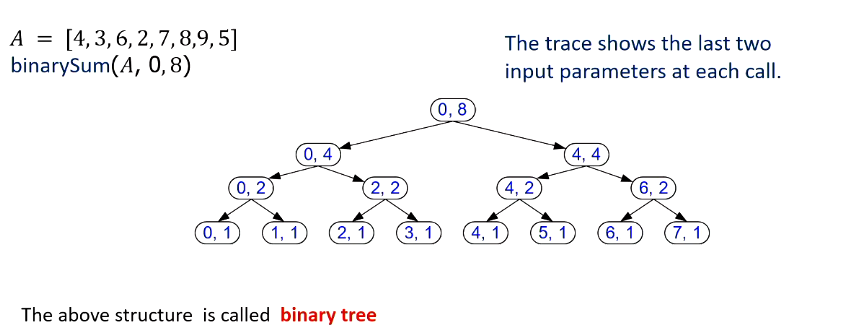
\includegraphics[width=0.8\textwidth]{figures/tree.png}
		\caption{Binary Tree}
		\label{fig:figures-tree-png}
	\end{figure}
\end{tcolorbox}
\subsubsection{Analysis}
The input is an array of size $k$. The time is proportional to the number of recursive calls as accessing elements and comparing are all of $O(1)$. The number of recursive calls, however, is running in $O(\log n)$ times. The remaining portion of the list of size is $\text{high} - \text{low}+1$. After one comparison, the number of candidate halves: 
\begin{align*}
	(\text{mid} - 1) - \text{low} + 1 = \left\lfloor \frac{\text{low} + \text{ high}}{2} \right\rfloor-\text{low} \le \frac{\text{high}- \text{low}+1}{2} \\
	\text{high} - (\text{mid}+1) +1 = \text{high} - \left\lfloor \frac{\text{low}+\text{high}}{2} \right\rfloor \le  \frac{\text{high}- \text{low} +1 }{2}
\end{align*} 
After $j$ th call, the number of candidates left is at most $\frac{n}{2^{j}}$. We need to have $\frac{n}{2^{j}}>1$ to have the algorithm running. 
\section{Heap}
A heap is a binary tree storing keys at its nodes and satisfying the following priorities:
\begin{itemize}
	\item Heap-order: for every internal node $v$ other than root, $key(v)\ge key(parent(v))$. 
	\item Complete binary tree: let $h$ be the height of the heap.
	\item The last node of a heap is the rightmost node of maximum depth.
\end{itemize}
A heap storing $n$ keys has height $O(\log n)$. For a heap based implementation of Priority Queue the idea is that we store a (key,value) elements at each node following that smaller key is higher priority. For insertion, let $k$ be the key element we insert to the heap. The insertion algorithm consists of three steps
\begin{itemize}
	\item Insert a new node $z$ (the new last node)
	\item Store $k$ at $z$.
	\item Restore the heap-order property
\end{itemize}
To restore, we use upheap
\begin{itemize}
	\item Algorithm upheap restores the heap-order property by swapping $k$ along an upward path from the insertion node
	\item The algorithm terminates when it is either at the root or a node whose parent has a key smaller than $k$
\end{itemize}
The running time for upheap is $O(\log n)$ due to its height. Removal, however, gets slightly tricky.
Recall removeMin() of the priority queue ADT. This means that removal of the root key from the heap.
\begin{itemize}
	\item Replace the root key with the key of last node $w$.
	\item We remove  $w$
	\item We restore the heap property using downheap
\end{itemize}
To restore, we use downheap
\begin{itemize}
	\item The algorithm swaps the parent node with it's children which is the smallest. 
\end{itemize}
With this, we bring heap sort
\begin{itemize}
	\item Sequence $S$, of $n$ elements
	\item Use PQ Sorting
	\item First phase we insert, one by one, the element in  $S$ to a priority queue $P$ 
	\item Second phase we extract the elements from $P$ by a series of removeMin()
	\item Put them back into $S$ 
	\item Now use a heap-based implementation for the priority queue
\end{itemize}
The performance of this is $O(n \log n)$.
\section{Skip-list}
Slip list is a set $S = \{ S_0,S_1,\ldots,S_h\}$. $S_0$ contains all elements, including $\pm \infty$. $S_i$ is a random subset of $S_{i-1}$ appear in $S_i$ with probability $\frac{1}{2}$, independently. $S_h$ contains only $\pm \infty$. To search, we start at the position of the top list. At the current position $p$, we compare $x$ with $y \le  key(next(p))$.
\begin{enumerate}
	\item $x=y$ we return element(next(p))
	\item $x>y$ we scan forward
	\item $x<y$ we drop down
\end{enumerate}
For insertion of an element $k$, we search for $k$ and find the positions $p_0,p_1,\ldots,p_i$ of the items with largest element $<k$ in each list $S_0,S_1,\ldots,S_i$. We work as in the search algorithm. To determine where we add, we toss a coin. Skip lists are implemented with quad nodes. I.e., it stores previous, next, above and below data. The issue with skip lists is that space usage is high. The space used by skip list depends on the random bits used by each invocation of the insertion algorithm. In our coin tossing, the probability of getting  $i$ consecutive heads is
\begin{align*}
	\left( \frac{1}{2^{i}} \right) 
\end{align*}
If each $n $ entries is present a set with probability $p_i$ the expected size of the set is $np$. 
\begin{align*}
	\sum_{j=0}^{\infty} \frac{n}{2^{j}} = 2n
\end{align*}
The expected space usage of a skip list with $n$ items is $O(n)$. The height with high probability, a skip list with $n$ items has height $O(\log n)$. The search time and update time is proportional to number of drop-down steps and the number of scan-forward steps. The drop steps are bounded by height $h$ of the skip list, i.e., $O(\log n)$ with high probability. The expected number of scan-forward steps is $O(\log n)$. Therefore it is $O( \log n)$.
\section{Binary Search Tree}
A binary tree storing keys at its internal nodes. External nodes do not store items. Property is for each internal $p$ with key $k(p)$, the key in the left subtree $<k(p)$. The right is $>k(p)$. Usually
\begin{itemize}
	\item $k(root) = k$ we found the element
	\item $k(root) < k$ $k$ must be on the right
	\item $k(root) > k$ $k$ must be on the left
\end{itemize}
If we reach a leaf, the key is not found. 
\subsection{Performance}
Consider a binary tree with $n$ items of height $h$. The space used is $O(n)$. Methods search,insert and remove take $O(h)$. The height $h$ is worst case $O(n)$. Best case is $O(\log n)$. 
\subsection{AVL Tree}
AVL trees are balanced regardless of the order we insert-delete elements of the tree. AVL tree is a binary search tree and for every internal node $v$ of $T$, the height of the children of $v$ can differ by at most $1$. The above is also known as the height balance property. The height of an  AVL tree storing $n$ keys is $O(\log n)$
\begin{proof}
	Let us bound $n(h)$: the minimum number of internal nodes of an AVL tree of height $h$. We can see that $n(1) = 1$ and $n(2) = 2$. For $n > 2$, an AVL tree of height $h$ contains the root node, one AVL subtree of height $h-1 $ and another of height $h-2$. That is, $n_9h) = 1 +n(h-1) + n (h-2)$. Knowing $n(h-1) > n(h-2)$ we get $n(h) > 2n(h-2)$. This implies $n(h) > 2^{\frac{h}{2}}>1$. Taking logarithms we obtain $h < 2 \log_n (h) + 2$ \\
	Insertion is as in binary search tree. Always done by expanding an external node. We call the balancing Trinode restructing. Let $(a,b,c)$ be the inorder listing of $x,y,z$. Perform the rotations needed to make $b$ the topmost node of the tree. 
\end{proof}
\end{document}






